\documentclass{article}
\usepackage{amsmath}
\usepackage{hyperref}
\title{Open RAN and the challenges in experimentation with open-source platforms}
\author{Gabriel}
\date{\today}

\begin{document}
\maketitle

\begin{abstract}
\end{abstract}

\section{Introduction}
    The Open RAN (O-RAN) architecture and the O-RAN Alliance specifications
    have the potential to promote virtualized and disaggregated Radio Access
    Networks (RANs), connected through open interfaces and optimized by
    intelligent controllers.

    Understanding the O-RAN architecture, interfaces and workflows is critical
    to the future of the telecommunications ecosystem. The evolution of O-RAN has
    many challenges due to its complexity, requiring experimental platforms to
    evaluate programmable and virtualized protocol stacks with the new open interfaces,
    in conjunction with RAN optimization within the 5G architecture and beyond.

    Our team at UnB spent quite some time looking for different platforms for
    experimentation and presented our findings, \cite{Solis_2022}, at the
    Brazilian Symposium of Telecommunications (SBRT2022).

    Since I didn't have any free time up till now and we didn't have enough space in the
    paper, lets review things here, were we can put any number of images.


\section{What do we need to get a working Open-RAN setup?}

    It isn't an official architecture diagram, but the diagram of the reference implementation
    made by the \href{https://wiki.o-ran-sc.org/display/OAM/OAM+Architecture#OAMArchitecture-IntegrationintoSMO}{O-RAN Software Community (O-RAN SC)}.architecture
    Figure \ref{fig:o-ran-sc-architecture} shows the main components of an O-RAN setup, which are:
    \begin{enumerate}
        \item the 3GPP core: 4G and 5G are supported in the O-RAN specifications (some companies are apparently adapting older networks too)
        \item the RAN components: the eNB or gNB, or its disaggregated counterparts (CU, DU, RU)
        \item the O-RAN components: near-RT RIC, non-RT RIC and the rest of the SMO, plus SDK for xApp/rApp development
    \end{enumerate}

    \begin{figure}
        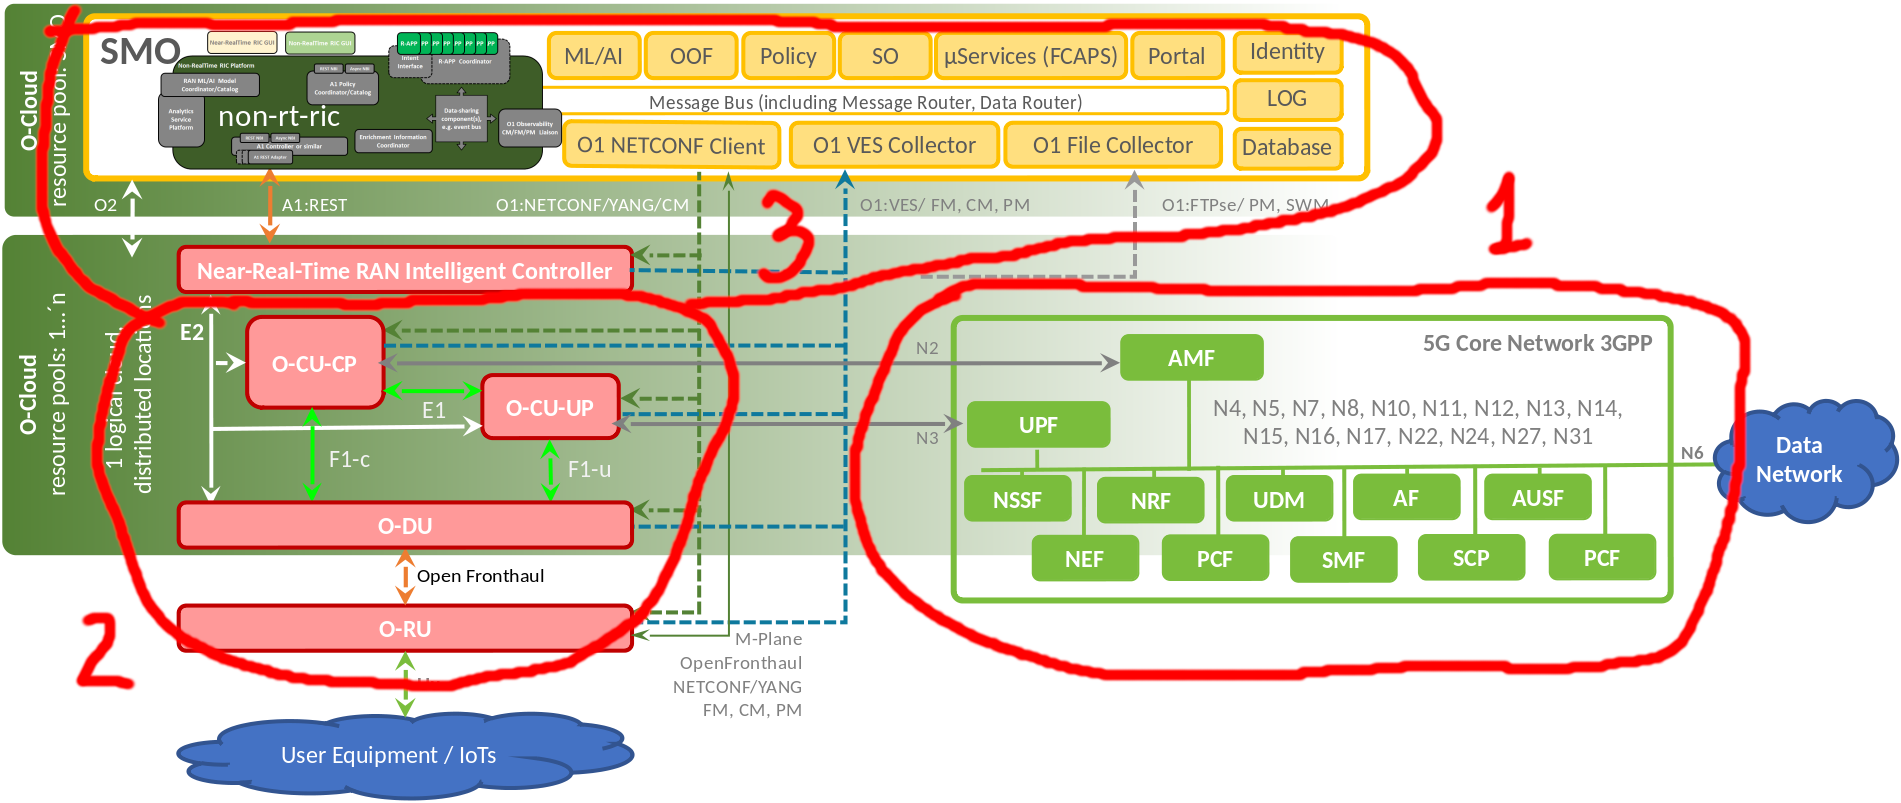
\includegraphics[width=1.0\textwidth,height=1.0\textheight]{"/assets/img/2022-12-22-experimental-platforms-for-open-ran/o-ran-sc-architecture.png"}
        \caption{Architecture diagram of the reference O-RAN implementation (the drawings are mine)}
        \label{fig:o-ran-sc-architecture}
    \end{figure}

    Let's look at each components alternatives.

    \subsection{5G Core implementations}

        We found two open-source implementations that are frequently used.
        The first one is the famous \href{https://openairinterface.org/oai-5g-core-network-project/}{OpenAirInterface-5G Core Network (OAI-5G CN)},
        which has been in the works for years and is used by a lot of researchers and companies,
        in both private and public networks.

        The second one is the \href{https://www.free5gc.org/}{free5gc}, which started as a fork
        of a 4G Core, \href{https://nextepc.org/}{NextEPC}, and continues to evolve. Also seems
        to be used on public networks.

        There are quite a lot of proprietary cores, but we can't be certain those are not
        forks of the open-source ones. To name a few companies and their cores:

        \begin{itemize}
            \item \href{https://www.ericsson.com/en/core-network/5g-core}{Ericsson - 5GC}
            \item \href{https://www.nokia.com/networks/core/5g-core/}{Nokia - 5GC}
            \item \href{https://www.tecore.com/core-network-products/}{Tecore – iCore}
            \item \href{https://capgemini-engineering.com/us/en/brochure/virtualized-next-generation-5g-core/}{Altran/Capgemini Engineering - Virtualized Next Generation 5G Core (ViNGC)}
            \item \href{https://www.mavenir.com/portfolio/mavcore/}{Mavenir – Mavenir Converged Package Core (MAVCore)}
            \item \href{https://carrier.huawei.com/en/products/core-network/sdm}{Huawei – SDM/PCC}
        \end{itemize}

        After we have a 3GPP core, we can then connect it to our RAN.

    \subsection{RAN implementations}
        Most likely due to complexity, performance issues due to signal processing overhead, and
        standards conformance and interoperability testing, there seems to be less options in terms of RAN.

        The eNB/gNB/CU/DU are available in open-source projects such as:
        \begin{itemize}
            \item \href{https://openairinterface.org}{OpenAirInterface}
            \item \href{https://www.srsran.com/}{SrsRAN}
            \item Radisys – gNB DU (part of the reference O-RAN SC implementation)
        \end{itemize}

        The O-RAN RICs and interfaces are available in open-source projects such as:
        \begin{itemize}
             \item \href{https://openairinterface.org/mosaic5g/}{OAI - FlexRic}
             \item \href{https://opennetworking.org/open-ran/}{Open Networking Foundation (ONF) - SD-RAN}
        \end{itemize}

        Other proprietary RAN implementations available:
        \begin{itemize}
            \item Radisys – ConnectRAN
            \item Huawei – SingleRAN
            \item Ericsson – Cloud RAN
            \item Nokia – AirScale Cloud RAN
        \end{itemize}

        And it is at this point someone asks me why I included Huawei in this list.
        The answer is: they can probably adapt their solution easily to support Open-RAN.
        As the time goes by, it will get even easier since all the tooling required for
        testing and conformance will be in place.
        If O-RAN really works and is set as a requirement in new spectrum auctions,
        they will certainly do it.

    \subsection{Orchestration and management (O\&M) services}
        This is where things really start to get big and ugly.

        We have great O\&M services such as \href{https://magmacore.org/}{Magma},
        which was started by Facebook, then moved to
        \href{https://telecominfraproject.com/}{Telecom Infrastructure Project (TIP)},
        and finally to Linux Foundation (stop moving the damned project around).

        Too bad it isn't comparible with O-RAN. Even then, it probably is one of the
        reasons O-RAN even became a thing, since TIP is also responsible for pushing
        O-RAN forward, along with Telcos, software/hardware/cloud partners and some governments.

        There is also \href{https://osm.etsi.org/}{Open-Source MANO}, which doesn't
        really seem to have gained much traction on the O-RAN space. But maybe I'm badly informed.

        \href{https://kubernetes.io/}{Kubernetes} on the other hand, seems to be the
        popular choice, since both \href{https://openairinterface.org/mosaic5g/}{Trirematics},
        OAI's O\&M solution, and the \href{https://opennetworking.org/open-ran/}{SD-RAN},
        ONF's O\&M solution, are based on Kubernetes.

        All of the services are implemented as Virtualized Network Functions (VNFs),
        that are executed within containers. The containers are glued together by
        software defined networks (SDNs). SD-RAN uses ONF's in-house SDN/NFV solution
        named \href{https://opennetworking.org/onos/}{ONOS}, while the reference
        O-RAN implementation uses Linux Foundation's
        \href{https://www.onap.org/}{Open Network Automation Platform (ONAP)}.

    \subsection{A blueprint}
        With all components at hand, we then need to sewn them together.

        This is when the problems really start appearing for a novice.

        There are quite a lot of components, all of them with different
        configuration settings, syntaxes and semantics. You have no idea
        what most of the settinds do and how to properly set them up, but
        you're still supposed to figure it out...

        You probably won't, because available documentation is pretty bad.
        I admit my documentation isn't up to par either, but that's how things are.

        We are supposed to believe \href{https://wiki.akraino.org/}{Akraino}
        blueprints work, but I haven't got a single one to work.
        Seems like another dead project from the Linux's Foundation.

        ONF is the most friendly one, with a complete and working blueprint,
        which they named
        \href{https://docs.sd-ran.org/master/sdran-in-a-box/README.html}{SD-RAN-in-a-box}
        , or just Riab.

\section{SD-RAN-in-a-box: a not so hidden gem}
    By far, SD-RAN-in-a-box is the most user-friendly Open-RAN solution.

    You just run a few commands and it setups everything up using the magic of
    good old Bash, Ansible, Kubernetes and ONOS.

    The user can select if they want to emulate the user data-plane. Which of course we want.

    It will create VM's running OAI that act like the eNB and UE, connected by a virtual channel.

    More surprisingly, since OAI is already running anyways, the user can choose to use a
    Software Defined Radio (SDR) to get a real network going.

    Of course the settings are meant for a lab setup, with very few UEs.

    There is a popular saying that says that the devil is in the details.
    I'd say that the devil is in the implementations.
    While the O-RAN standard look fairly simple, the implementation complexity
    can vary wildly depending on the implementer choices.

    When I found SD-RAN-in-a-box, I started looking at the settings to understand how
    exactly it worked, what was connected to what, which standard defined the different interfaces.

    Ended up writing a MermaidJS diagram. But since is too big to show, here is the \href{https://mermaid-js.github.io/mermaid-live-editor/edit#pako:eNqdWftvozgQ_lesnFa605VNeGS77f2U5tHNbQsRCdKe6GlFwU1RiUE8uu1t93-_8YPEEJISIiUQz_fZ4xnPeDA_e34c4N5lb516ySNaTe4Igs-HD2iJ0-fQx-jWI94abzDJkUcCZKX-I87y1MvDmCA_3iQxAVnGeVlxzzta3lq8pdJqLZdXy6Vb7YP2Kg0ixs3Qv7sO6McyreX4Zu7SK4KbfkziTPGjsAl47Qgg3HDgutgDfnWuprY5XU2X7tfiHqcE5zAsVcePSe6FBKeNWliLqT1aWTYfwUowTCRO-TCx-NfEW9jWt384aZHGL6-ckdDbOjzLXyNcThk9hFF0-dswuD9XjUM4mOi7uN2EW3VZzrMVmE3uCFLMRVEUSYtGx1UghzwGoDfJaaPFHL3JOh_2GmWOkmTrN85j6ldJUUielmx-A5hnGj_hcmZn_K_yIwzyx8th8vLXIabamal1ZuonMDEJ7sjuL0Ttd0tdufCVVyRr1qBZY807AaSJkOQ4ffBowHopRiTOYXiIIS8Nwv9wcIY834_hnqxRHleYlmKPTGTGRLFXyJ6PL9GsID5NCV6ERpAiwhz7eQGdqh8H6o5aWQS2ujogEXM5JtUk6c5-xgn227GGnVifWrBqBi8N5hE0B9tHUbimaXMMKSuNowinDXnXtOwVWNjdGbuecATi-wi8P6p6n37AzK6935xCIKku--0ncRT6r2izy-SZ2EEaSBojaX1M0tB_ZOiQPMTphm8JDQydMfT-7Q3awI4VyQNV1qQw0ziOILZ3-xPyMlSQAKcowM84ihPGBEh9xTYlODr195Igm5BAzWbGQL04hNKPoGAkmqBsFb1JLjmIYaY_KtWOSvW65XZL87xzAvrcmXnRPdEOTs16lZta9WJBZoJMMXPMsQv7BOGZCuc_4vRpm6UqtQENTOylio0hea3CDaZB1hCJIg4ZdC8QRfDxusBTc1k2hfwLXy7DWkUmUraoiGLyEK5lsTM151euM1XgwjEFJuG9DFlZC8tNFWjlgDxOYln-wgKd_XLAUxJuqoH6wsKa_XJImm3qcp3JdS7fPO4NYTC5IeTRfV0-ZPKhKJz8SkUnhQvb4tX-3xlo-Bx66EueJ-itEkdid6BIS-1_g6xCgeDzsWXOoCSQsdv6gKLnBJJFFGXgEMRLtywMsO-lOexvrDEOMvQ21WodyOXHCqwbxevXXQ0CPSXe2qOlTF4K_UePrKGBKra2F2P0Rr0kB6y0_HeFxsO5Gtxr7bYfVetG0zttdqrRareTooEaiwdDEkp2eKlmPasJaN7OTwRqbYF6W6DRFjisRdqBeXP_t0GykG8HraxUZoe2QL0t0GgLHLYBSguqW9GlfupGO-9G-9yNdtGJpg260dRuNK0brVv-0LpV5lq3VaJ1WyXaeffHr12VMDIrpQVsKyYUvRn6HZtX6E_IHFdo7IibifOH1KN55cK3b43m1bJ42zdQoPIN81eXkuvnDhJq7Eg4GK0GpR-GGi8EQhkv2LhkRh_HjzCcLcORGc6iztjWZ036TWT9Js7-U4AYb-IIhDTUxDk6VOUPkG3ehV1h8YKeSUVB76nGIAj2ntgsVXpKbl2CgBdbY4UfTsM7J-EnTuNq_9ypgNAuOtH0QTfaKcVRPe6aPAfbEbXUVOuPluZHldlqOV4tak47DNvz1ztQpy202Ut6tzJP17vRjG60YQta1TtSXLGO6CGTz89BaDFeZDhVksgjuBLM1PLMgmqDdSV9Pkn6ePdq0OJsZiZp1DjmTFX8PUcJJYS8OObI8xY6NdA-t5qKnLLoQ-8sBVt-8YqoMQiYkixhMOwXSOdLZUGtzSZgO0egtweA1fPd99DSBLvlE6NbPjFOySfVs4bytKF23uDASp3gZ5deEdzI7z_AG86U3zpTeIqXN8xpCYK8Qy12k2PFKWj5z5uZwaiArOvtk6Z2aY5ay5UmUfTTKUZLimS8rdFWjynG14vFOE6xq8PN9oSGtjQf09yspmPLnrpwVUZ945pDj57smNeMQdb9YRu4GIEad6myl0nftNq-wHukCPMa0gHDEJEXqttCBVmUyOJo3jKGnXKE8akb7fyk1FIJcGGqA1I-98Yxuz1RGW2fqKTFZo1vLGfiWso4ioug9LN4ecByFDiXg-prezhovZ9BiN_g9TZTbFe43BiEKWarDa3EUqKHlPMyMe-OKbdNpbZlnOywLFj2cPNNEi0T7Lv0hh2ss8N4hbaFD6Ff4sw4pwgXrigsoTiQxMvcI0yc5V55rF6KK1qDBfe0O6A0QEsFq-rSpcI1qqjHm6km28TB31XK44u6nftHRu0Nv0XSNS4jSzUa3g9wgNCn9ohQkVMtG94JSGup3HHE4hk05NKh1gKjt8AYTZhtZPTOehucbrww6F32ftLmu17-CGvgrncJt-Dup7veGW-nf27huZWK8rQA1_4CepEEXo6nQZjHae-Stp_1vCKPl6_E710-eFGGS9Ak9CASNqL11_-INcE4}{link}.

    \subsection{Stop the talking and show us some code!}
        \subsubsection{Installation}

            Well, if you follow the manual, you will get there.

            At the time I tested things, only Ubuntu 18.04 was supported.
            Later versions will fail with a nf\_conntrack issue, so you may need to run everything in a VM.

            Running things in a VM can also create problems, but more on that later.

\begin{verbatim}
# Check if you have virtualization support
sudo modprobe kvm
lsmod | grep kvm

# Check if you have AVX2 (a flavor of SIMD for floating point operations)
egrep "(avx2)" /proc/cpuinfo

# Check if you have virtualization instructions
egrep "(svm|vmx)" /proc/cpuinfo

# Don't even try to continue if one of the
# previous checks didn't return something

# Clone Riab
git clone "https://github.com/onosproject/sdran-in-a-box.git"

# Install Vagrant (VM manager) and the libvirt extension
apt install vagrant qemu-kvm libvirt-daemon-system

# Create a new Ubuntu 18.04 VM
vagrant init "generic/ubuntu1804" # bionic64

# Edit the vMemory and vCpus for the machine
# If you use the emulated data-plane, use >22GB of RAM
#
#  # -*- mode: ruby -*-
#  # vi: set ft=ruby :
#  Vagrant.configure("2") do |config|
#    config.vm.box = "generic/ubuntu1804" #
#    config.vm.synced_folder "./", "/vagrant" # sync the local directory to the VM's /vagrant directory
#    config.vm.provider "libvirt" do |vb|
#      #vb.gui = true
#      vb.cpus = 14
#      vb.memory = "21384"
#    end
#    config.ssh.insert_key=false # passwordless login
#  end

# Start the VM
vagrant up

# Log into the VM
vagrant ssh

# Update packages
sudo apt-get update
sudo apt-get upgrade

# Lock the kernel version. It might not be a problem on every cloud,
# but it was on mine.
sudo apt-mark hold linux-generic linux-image-generic linux-headers-generic

# Install extra kernel modules (nf_conntrack)
sudo apt install linux-modules-extra-*-generic
sudo modprobe nf_conntrack
sudo apt-get install make net-tools

# Nagivate to the cloned SD-RAN-in-a-box directory
cd /vagrant/sdran-in-a-box
\end{verbatim}

            Now, how do we do anything?

        \subsubsection{Basic Helm/Kubernetes background information}
            I'm definitely not an specialist in SD-RAN, Kubernetes or ONOS,
            so it took some experimentation to get anything done.

            \href{https://helm.sh/docs/intro/using\_helm/}{Helm charts} are used as an encapsulation
            for kubernetes applications along which can be configured using templates for the
            different settings. It is just as bad as it sounds.

            Helm charts can have subdirectories, which are considered subdependencies and are installed recursively.

            A helm chart can be installed from a local repository (so you can work on a local clone)

\begin{verbatim}
helm install oai-enb-du sdran-in-a-box/workspace/sdran-helm-charts/oai-enb-du
\end{verbatim}

            The templated settings allow for the substitution of values via the command line
            or via yaml files (much preferred).

\begin{verbatim}
echo '{
 config.oai-enb-du.mode: "nfapi",
 config.oai-enb-du.radio.eutra_band: 42,
 config.oai-enb-du.radio.rbs: 100,
 config.oai-enb-du.radio.tx_gain: 90,
 config.oai-enb-du.radio.rx_gain: 125,
 config.oai-enb-du.radio.nb_antennas_rx: 2,
 config.oai-enb-du.radio.nb_antennas_tx: 2
}' > values.yaml
helm install -f values.yaml oai-enb-du sdran-in-a-box/workspace/sdran-helm-charts/oai-enb-du
\end{verbatim}

            In this case, one of the templates in sdran-in-a-box/workspace/sdran-helm-charts/oai-enb-du/templates/*.tpl
            will have their field values replaced with those in the yaml settings file.

            For example, in the values file, we set "oai-enb-du.mode" to "nfapi", which will be processed
            by the following template:

\begin{verbatim}
{{ $duMode := index .Values "config" "oai-enb-du" "mode" }}
\end{verbatim}

            and transformed into the following line

\begin{verbatim}
duMode := "nfapi"
\end{verbatim}


            The helm charts used by the SD-RAN-in-a-box are installed by
            the makefiles em sdran-in-a-box/mk, using the following commands

\begin{verbatim}
helm upgrade --install $(HELM_ARGS) \
     --namespace $(RIAB_NAMESPACE) \
     --values $(HELM_VALUES) \
      ...
\end{verbatim}

            The values of HELM\_VALUES are read from the default settings file
            sdran-in-a-box/sdran-in-a-box-values.yaml

            To install from your own sdran-helm-charts fork, replace the repository link in
            sdran-in-a-box/Makefile. To do that, search for

            \begin{verbatim}
            $(ONOS_GITHUB_URL)/sdran-helm-charts
            \end{verbatim}

            The clone is only done if the directory does not exist, so you can modify it
            directly, then commit and push changes later. Just remember to do that before
            running "make clean-all", otherwise the changes will be lost.

        \subsubsection{Installing RIAB with data-plane emulation}
            If you do not have enough RAM, the VM or your computer will crash due to OOM.

\begin{verbatim}
# Install RIAB with OAI emulation
make OPT=oai

# Execute tests to check if the data-plane is actually working
# Tests are located in sdran-in-a-box/mk/test-cases
# E2E tests using pings in the user data-plane
make test-user-plane

# E2E tests using iperf in the user data-plane
make test-rsm-dataplane
\end{verbatim}

            Everything should be working now. You must be thinking on passing quite
            some traffic through that emulated network right now, but it isn't that simple.

            At least on my computer, due to using a normal kernel (not the low-latency one),
            and due to low CPU clocks (1st gen Ryzen 1700), the synchronization between the
            UEs and the eNB is lost quite frequently. I remember looking at the ONF Slack
            channel for answers, but it was still being investigated.

            Due to that issue, I had to take everything down and up again, which took quite
            a lot of time. I tested the commands suggested by Woojoong Kim (I believe he is
            the lead developer for Riab), but didn't really work for my specific case.

\begin{verbatim}
# I only really use clean-all, because it always works. Beware: it is super slow and deletes everything

# It deletes ONOS RIC services and RAN-Simulator but Kubernetes is still running
make reset-test

# Deletes Kubernetes environment; Eventually, all ONOS RIC and
# RAN-Simulator are terminated; The Helm chart directory is not deleted

make clean

# Deletes everything, including the Kubernetes environment,
# all componentes/PODs which RiaB deployed, and even the Helm chart directory

make clean-all
\end{verbatim}

        \subsubsection{Other useful commands}
            Other useful commands I've learned while testing these.

\begin{verbatim}
# Lists all kubernetes namespaces and services
kubectl get po --all-namespaces

# Lists kubernetes services in the riab namespace
kubectl -n riab get pods

# Lists the status of sd-ran
helm -n riab status sd-ran

# Lists all sd-ran settings
helm -n riab get all sd-ran

# Check the status of different pods running SD-RAN services
watch kubectl -n riab get pods

# Comand to get the kubernetes pod shell to access binaries
kubectl -n riab exec -it $(kubectl -n riab get pods -l type=cli -o name) -- /bin/sh
\end{verbatim}

    \subsection{That's enough code. Now show us something interesting}
        I wish I had some banging xApps up and running... Maybe getting to work in real
        networks with people from Mavenir, Parallel, Radisys or Nokia...

        But in my excitement about this, I ended up talking too much and getting a ton
        of people wanting to get envolved, which ended up drastically slowing down the process.

        A few partners offered us their clouds, which I'm very grateful for, but they were quite
        up to the task of running real-time services. Some failed to setup Riab due to missing AVX2
        instructions, others due to disabled smx/vmx instructions for security reasons, others
        had very slow drives which timed out some of the services and prevented Riab from getting
        setup. Even if they worked, I'm not sure their clocks and number of cores would be able to keep up
        with the emulated network.

        I also had my fair of issues trying to understand Helm packaging.

        The best I managed to do was adapt our in-house traffic injection tool,
        \href{https://github.com/notopoloko/Eros}{Eros}, and use it
        to  \href{https://github.com/Gabrielcarvfer/sdran-in-a-box/blob/work/inject_eros_traffic.py}{inject}
        some network traffic and see how things behaved. We produced the Figure \ref{fig:traffic-injection},
        showing the behavior of the UE downlink when streaming a MPEG DASH-like traffic from the remote serve.

        \begin{figure}
            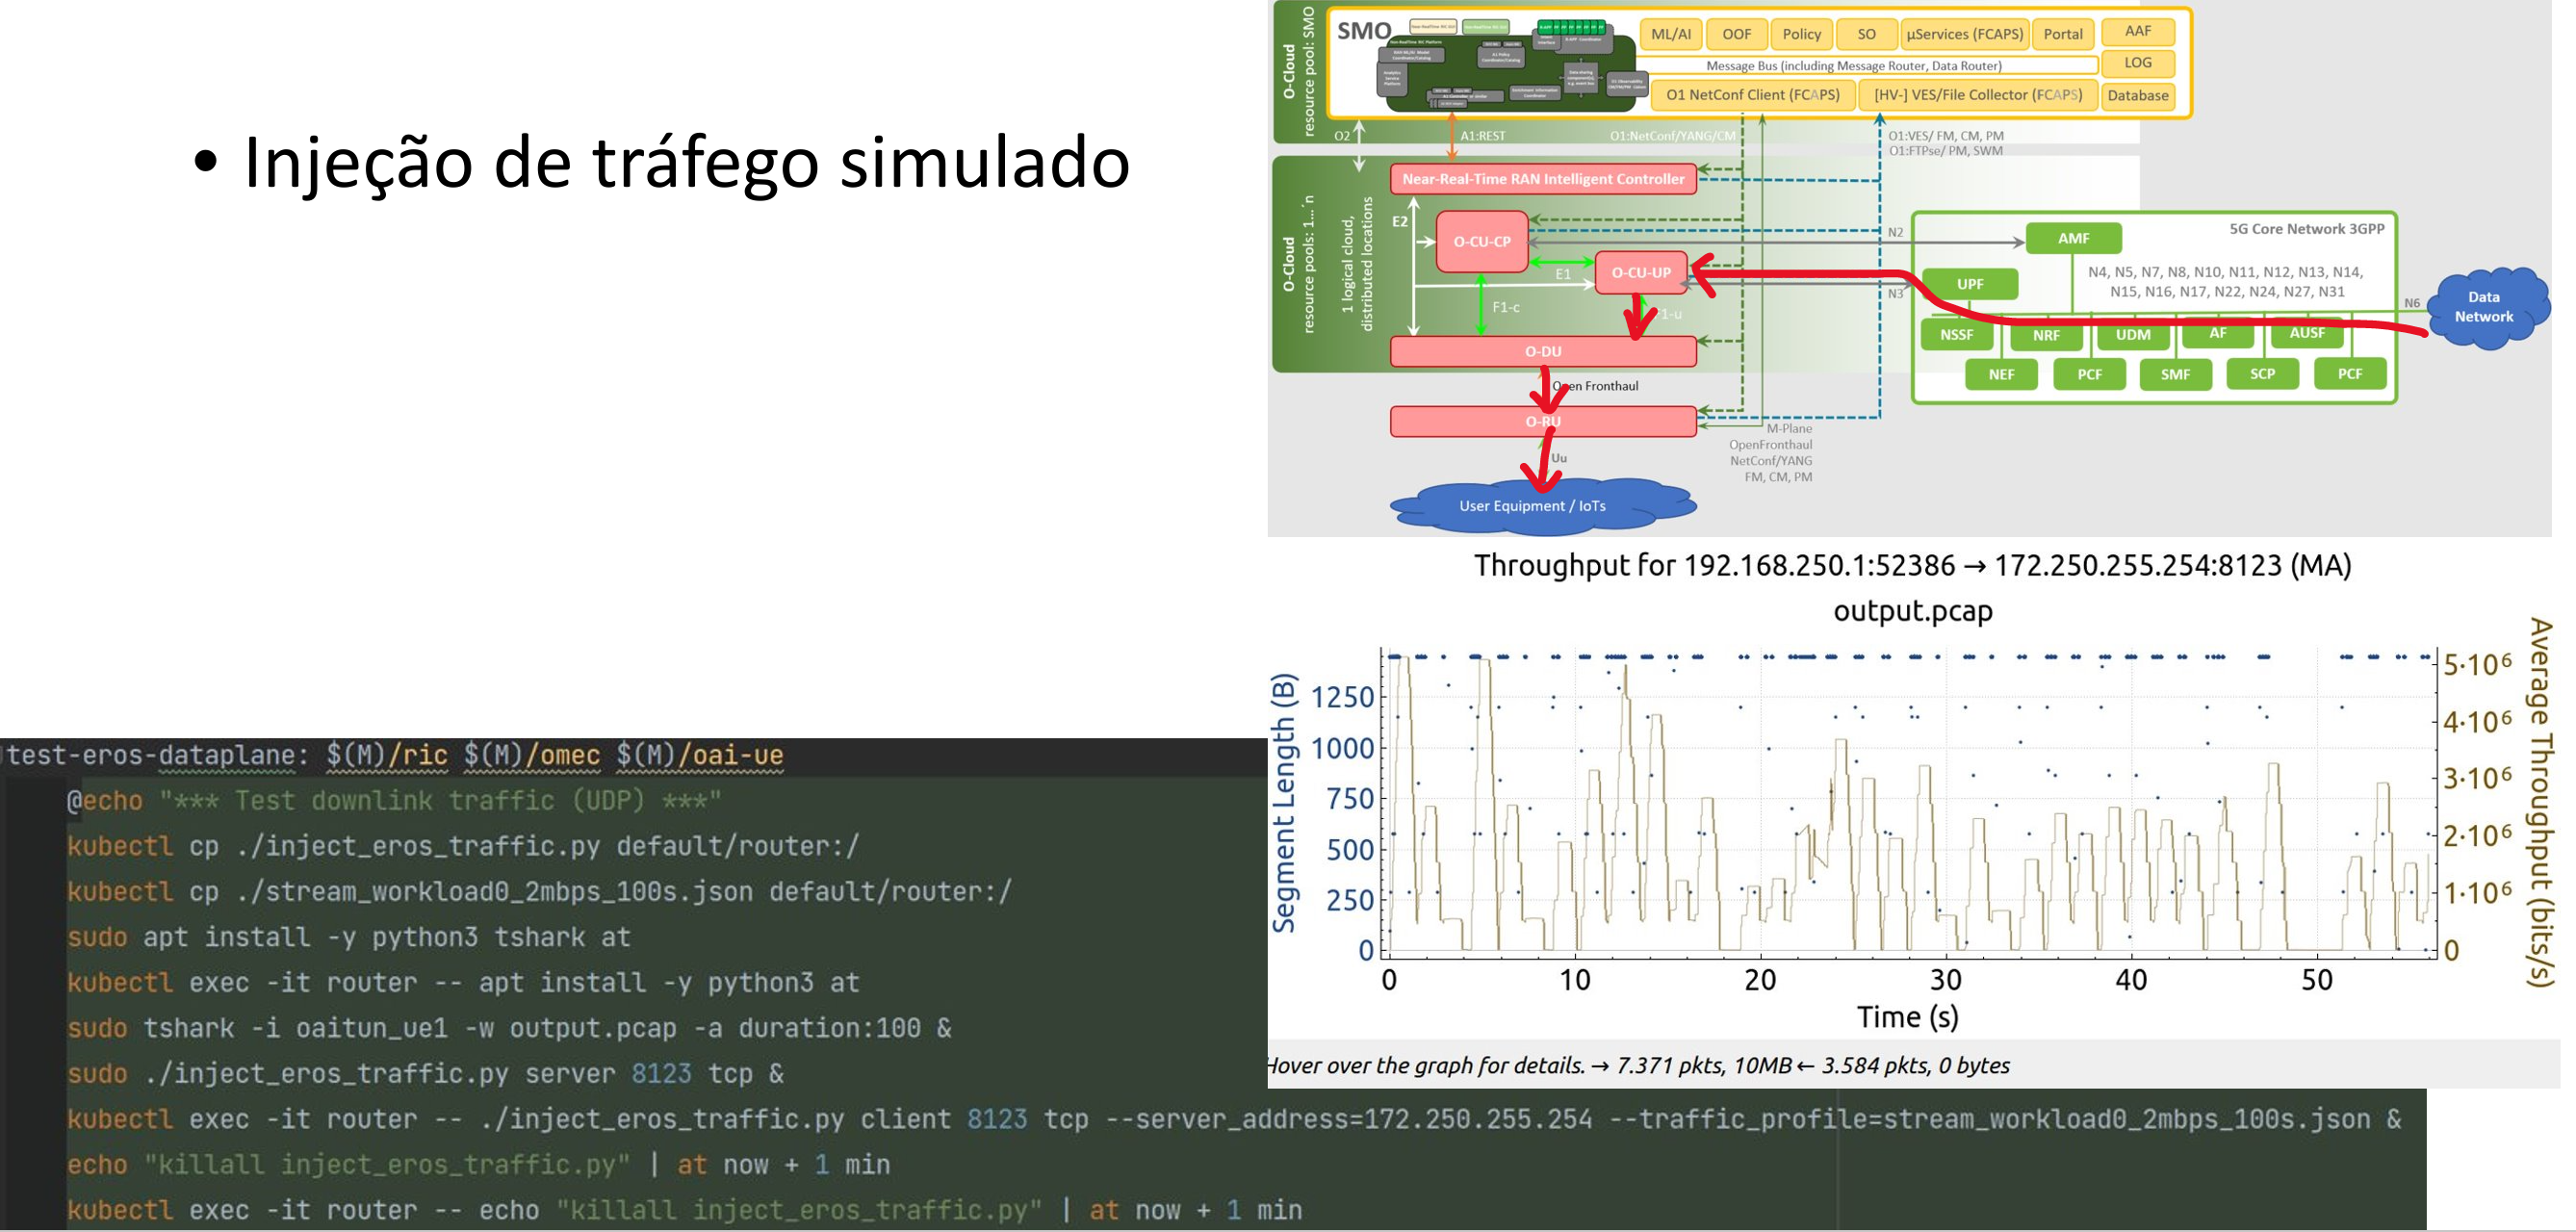
\includegraphics[width=1.0\textwidth,height=1.0\textheight]{"/assets/img/2022-12-22-experimental-platforms-for-open-ran/traffic-injection-sdran.png"}
            \caption{Traffic injection from the remote server to the UE using the emulated data-plane}
            \label{fig:traffic-injection}
        \end{figure}


\section{Next steps}
    For now, I've stopped playing with SD-RAN and started focusing on my own O-RAN implementation
    for the ns-3 simulator.

    It is kind of sad that I decided to change course too late and missed the
    \href{https://www.comsoc.org/publications/journals/ieee-jsac/cfp/open-ran-new-paradigm-open-virtualized-programmable-and}{journal}
    I had in mind.

    Hopefully it will make it to the Brazilian Symposium of Computer Networks and Distributed Systems (SBRC),
    which funnily enough will be hosted by my alma mater, in the next year.

    The source code for my O-RAN module should be published in a month or so, before I finish the paper for the
    tools section of the SBRC. It still needs some refactoring to look decent.

\section*{References}
\end{document}